\introparte{El Prolegómeno sitúa el trabajo. El capítulo~\ref{cap:introduccion}
presenta la motivación, los objetivos y el alcance de PymeKit; el
capítulo~\ref{cap:contexto} analiza qué necesitan las pymes, el estado de la
técnica y la justificación de la solución; y el capítulo~\ref{cap:plan}
recoge el plan de gestión del proyecto: metodología, tecnologías,
planificación, organización, costes, riesgos y aseguramiento de la calidad.}

\chapter{Introducción}
\label{cap:introduccion}
% ------------------------------------------------------------------------------
% Capítulo 1 · Introducción
% Fuentes: propuesta aprobada del TFG (objetivo, descripción, alcance y EDT),
% docs/tfg/{PLAN,REQUISITOS,DECISIONES}.md.
% ------------------------------------------------------------------------------

Este capítulo presenta la motivación del trabajo, sus objetivos y su alcance,
tal como se fijaron en la propuesta aprobada, y describe la organización del
resto del documento.

\section{Motivación}
\label{sec:intro-motivacion}

Las pequeñas y medianas empresas constituyen la inmensa mayoría del tejido
empresarial europeo~\cite{ec-sme-definition}. Para muchas de ellas, disponer
de una aplicación web propia ---una tienda, una zona de clientes, un sistema de
reservas o una herramienta interna--- ha dejado de ser opcional. El modelo de
\textit{Software as a Service} (SaaS)~\cite{nist-cloud}, en el que la aplicación
se ofrece a través de la red y se paga por uso o por suscripción, es la forma
habitual de construir y explotar este tipo de productos.

Sin embargo, cualquier aplicación SaaS, por sencilla que sea su lógica de
negocio, necesita un conjunto de piezas que se repiten de un proyecto a otro:
registro e inicio de sesión con verificación de correo y segundo factor,
cuentas de usuario y de organización, invitaciones y roles, cobro de
suscripciones, una consola de administración y alguna forma de consultar y
corregir los datos sin escribir consultas a mano. Ninguna de ellas aporta
valor diferencial al producto, pero todas tienen que estar bien hechas: un
error en el control de acceso o en el aislamiento entre clientes compromete
los datos de todas las empresas que usan la aplicación.

Para un equipo pequeño, o para un desarrollador que da servicio a varias
pymes, construir estas piezas desde cero en cada proyecto es lento y
arriesgado. Lo razonable es partir de una base común, ya probada, y dedicar
el esfuerzo a lo que distingue a cada producto. Esa es la idea que motiva este
trabajo: disponer de una \textbf{arquitectura software reutilizable} que
reduzca el tiempo de puesta en marcha de nuevos productos SaaS, facilite la
reutilización de componentes comunes y estandarice buenas prácticas en
seguridad, gestión del acceso, persistencia de datos y administración del
sistema.

\section{Objetivos}
\label{sec:intro-objetivos}

\subsection{Objetivo general}

El objetivo general, tal como figura en la propuesta aprobada, es
\emph{diseñar, implementar y validar una arquitectura software reutilizable
que sirva como base para el desarrollo ágil de aplicaciones SaaS orientadas a
pequeñas y medianas empresas, integrando los componentes esenciales de una
solución moderna: \textit{frontend}, \textit{backend}, sistema de
autenticación, gestión de usuarios y roles, integración de pagos y un módulo
CMS para la administración de contenidos y datos.}

\subsection{Objetivos específicos}

A partir de la descripción y del alcance de la propuesta, el objetivo general
se descompone en los objetivos específicos de la
tabla~\ref{tab:intro-objetivos}. Cada uno se relaciona con los requisitos del
capítulo de Requisitos del Sistema y se retoma en las conclusiones
(capítulo~\ref{cap:conclusiones}) para valorar su grado de cumplimiento.

\begin{table}[htbp]
  \centering
  \small
  \caption{Objetivos específicos del trabajo y requisitos relacionados.}
  \label{tab:intro-objetivos}
  \begin{tabularx}{\textwidth}{@{}lXl@{}}
    \toprule
    \textbf{ID} & \textbf{Objetivo específico} & \textbf{Requisitos} \\
    \midrule
    OE-1 & Analizar el contexto de las aplicaciones SaaS para pymes, identificar los componentes comunes reutilizables y definir los requisitos funcionales y no funcionales de la plataforma base. & Todos \\
    OE-2 & Diseñar una arquitectura modular que separe \textit{frontend}, \textit{backend}, base de datos y servicios auxiliares, con paquetes desacoplados. & RF-01, RF-02, RNF-04 \\
    OE-3 & Diseñar e implementar la autenticación, la autorización y la gestión de usuarios, equipos y roles, aplicando el control de acceso en la propia base de datos. & RF-03--RF-06, RNF-02, RNF-03 \\
    OE-4 & Integrar una pasarela de pagos para la gestión de suscripciones. & RF-07 \\
    OE-5 & Integrar un módulo CMS para la administración de contenidos y de los datos almacenados, con permisos propios y auditoría. & RF-08--RF-11 \\
    OE-6 & Diseñar un modelo de datos multicliente (\textit{multi-tenant}) con relaciones, restricciones y mecanismos de acceso orientados a la reutilización. & RNF-02, RNF-03 \\
    OE-7 & Preparar la plataforma para su reutilización: configuración centralizada, estructura de proyecto reproducible e interfaz en español extensible a otros idiomas. & RF-13, RNF-01, RNF-05 \\
    OE-8 & Validar la solución con pruebas de los principales casos de uso y de la integración entre módulos, y evaluar su reutilización en un escenario de ejemplo. & RNF-01, RNF-06 \\
    OE-9 & Definir el despliegue y elaborar la documentación: memoria, documentación técnica y manuales de instalación y de uso. & RNF-07 \\
    \bottomrule
  \end{tabularx}
\end{table}

\section{Alcance}
\label{sec:intro-alcance}

La propuesta organiza el trabajo en una Estructura de Descomposición del
Trabajo (EDT) con seis paquetes: (1)~análisis del problema y definición de
requisitos; (2)~diseño de la arquitectura software; (3)~diseño del modelo de
datos; (4)~implementación del prototipo funcional; (5)~validación de la
solución; y (6)~documentación. Los entregables comprometidos son la memoria,
el software desarrollado, los ficheros de configuración y despliegue, el
manual de instalación y puesta en marcha y un manual básico de uso. La
relación entre los paquetes de la EDT y las fases reales del proyecto se
detalla en el plan de gestión del proyecto (capítulo~\ref{cap:plan}).

El prototipo debe incluir, como mínimo, gestión de usuarios, autenticación,
persistencia de datos, administración desde un panel CMS e integración con un
flujo de pago. Dentro de ese marco, a lo largo del proyecto se fijaron estas
decisiones de alcance:

\begin{itemize}
  \item \textbf{Plataforma genérica.} PymeKit es una base reutilizable, no
        una aplicación de un sector concreto. Su configuración por defecto
        corresponde a la web de \emph{una} pyme: página pública y blog,
        acceso de clientes y personal, pagos y una consola de administración
        (ADR-005, ADR-020). Los equipos y las suscripciones se conservan
        como módulos que cada instalación activa si los necesita.
  \item \textbf{Un único CMS, de datos.} La propuesta pide un CMS para la
        administración de contenidos y de datos. Se cubre con un CMS que
        trabaja directamente sobre las tablas de la base de datos. El
        contenido editorial (el blog) se guarda también en la base de datos y
        se gestiona desde ese mismo CMS, en lugar de mantener un segundo gestor
        de contenidos basado en ficheros (ADR-004, ADR-017).
  \item \textbf{CMS integrado en la consola.} El CMS no es una aplicación
        aparte: forma parte de la consola de administración de la web, con un
        solo servicio y un solo inicio de sesión (ADR-011).
  \item \textbf{Interfaz solo en español}, sin textos escritos directamente
        en el código, de modo que añadir otro idioma sea un punto de
        extensión documentado (ADR-021).
  \item \textbf{Fuera de alcance:} aplicaciones móviles nativas, la lógica
        de negocio de un sector concreto, la facturación fiscal (emisión de
        facturas con validez legal) y la explotación en producción con
        clientes reales. Los pagos funcionan en el modo de pruebas de la
        pasarela.
\end{itemize}

\paragraph{Aportaciones del trabajo.}
Las aportaciones del trabajo son:

\begin{itemize}
  \item la \textbf{integración del CMS} en la consola de administración de la
        web (ADR-011): montaje de su API dentro del servidor web, pantallas
        implementadas como rutas de la aplicación, sesión única y control de
        acceso coordinado entre los permisos de la plataforma y los del CMS
        (ADR-014, ADR-016) y una sola base de datos para ambos (ADR-012);
  \item la \textbf{unificación de la pila} de librerías de formularios,
        textos y componentes de interfaz en toda la web (ADR-013);
  \item la \textbf{interfaz en español} sobre una infraestructura de
        internacionalización extensible (ADR-021);
  \item la \textbf{consola por áreas de negocio}, con nombres en español
        para las tablas, ayudas contextuales en los formularios y un resumen
        en cada pantalla (ADR-020);
  \item la \textbf{auditoría adversarial y corrección documentada de fallos
        de seguridad}, fijados con pruebas de regresión (ADR-015 y bitácora
        de incidencias);
  \item la \textbf{configuración reutilizable} centralizada, el
        \textbf{despliegue} y la \textbf{documentación} técnica y de usuario.
\end{itemize}

\section{Glosario de términos}
\label{sec:intro-glosario}

\begin{description}[style=nextline,leftmargin=1.2cm]
  \item[AAL (\textit{Authenticator Assurance Level})] Nivel de garantía de
        una sesión: \texttt{aal1} tras la contraseña o el enlace mágico;
        \texttt{aal2} tras verificar además un segundo factor.
  \item[ADR (\textit{Architecture Decision Record})] Registro breve de una
        decisión de arquitectura con su contexto, alternativas y
        consecuencias~\cite{nygard2011adr}.
  \item[BaaS (\textit{Backend as a Service})] Servicio que ofrece ya
        construidos la base de datos, la autenticación, el almacenamiento y
        una API, de modo que la aplicación no necesita un \textit{backend}
        propio para esas funciones.
  \item[CMS (\textit{Content Management System})] Sistema para gestionar
        contenidos. En este trabajo, un CMS \emph{de datos}: una interfaz para
        consultar y editar las tablas de la base de datos con permisos.
  \item[E2E (\textit{end-to-end})] Prueba que ejercita la aplicación completa
        a través de un navegador, como lo haría un usuario.
  \item[EDT] Estructura de Descomposición del Trabajo (\textit{Work Breakdown
        Structure}).
  \item[i18n] Internacionalización: preparar el software para mostrar sus
        textos en varios idiomas sin modificar el código.
  \item[MFA (\textit{Multi-Factor Authentication})] Autenticación con más de
        un factor; aquí, contraseña más un código temporal (TOTP).
  \item[Monorepo] Repositorio único que contiene varias aplicaciones y
        paquetes con dependencias explícitas entre ellos.
  \item[Multi-tenant (multicliente)] Arquitectura en la que una sola
        instalación da servicio a varios clientes (\textit{tenants}) cuyos
        datos deben quedar aislados entre sí.
  \item[pgTAP] Marco de pruebas unitarias para PostgreSQL~\cite{pgtap}.
  \item[Pyme] Pequeña y mediana empresa: menos de 250 personas empleadas y un
        volumen de negocio anual de hasta 50 millones de euros o un balance
        de hasta 43 millones~\cite{ec-sme-definition}.
  \item[RBAC (\textit{Role-Based Access Control})] Control de acceso basado
        en roles a los que se asignan permisos.
  \item[RLS (\textit{Row Level Security})] Mecanismo de PostgreSQL que filtra
        las filas que cada usuario puede leer o modificar mediante
        políticas~\cite{postgresql-rls}.
  \item[SaaS (\textit{Software as a Service})] Modelo en el que el proveedor
        ofrece una aplicación a través de la red sobre una infraestructura
        que gestiona él mismo~\cite{nist-cloud}.
  \item[\textit{Server function}] Función que se ejecuta en el servidor pero
        se invoca desde el cliente como una llamada tipada.
  \item[Super-admin] Administrador de la plataforma, con acceso a la consola
        y a todos los permisos del CMS.
\end{description}

\section{Organización del documento}
\label{sec:intro-organizacion}

La memoria sigue la estructura de la plantilla de la Escuela Superior de
Ingeniería y se divide en cuatro partes:

\begin{itemize}
  \item \textbf{Prolegómeno.} Este capítulo de introducción; el
        capítulo~\ref{cap:contexto}, de antecedentes, con la situación de las
        pymes ante el software SaaS, el estado de la técnica y la
        justificación de la solución; y el capítulo~\ref{cap:plan}, con el
        plan de gestión del proyecto: metodología, tecnologías,
        planificación, organización, costes, riesgos, gestión de la
        configuración y aseguramiento de la calidad.
  \item \textbf{Desarrollo.} Los capítulos de requisitos, análisis, diseño,
        construcción, pruebas y despliegue del sistema, que recorren las
        etapas del proceso de ingeniería con los diagramas, las decisiones y
        los fragmentos de código más significativos.
  \item \textbf{Epílogo.} Las conclusiones (capítulo~\ref{cap:conclusiones}),
        con el grado de cumplimiento de los objetivos, las lecciones
        aprendidas y el trabajo futuro; la información sobre la licencia y la
        bibliografía.
  \item \textbf{Anexos.} El manual del desarrollador
        (anexo~\ref{cap:manual-desarrollador}), el manual de instalación y
        puesta en marcha (anexo~\ref{anx:manual-instalacion}), el manual de
        usuario (anexo~\ref{cap:manual-usuario}) y la evaluación de la
        reutilización de la plataforma (anexo~\ref{cap:evaluacion}).
\end{itemize}

El software se entrega como un repositorio git con el monorepo completo:
código de la aplicación y del CMS, esquemas, migraciones y pruebas de la base
de datos, pruebas de extremo a extremo, configuración de integración continua
y de despliegue, y la documentación interna del proyecto (plan, requisitos,
decisiones, trazabilidad y bitácora). El repositorio es privado (véase la información sobre
licencia).



\chapter{Antecedentes}
\label{cap:contexto}
% ------------------------------------------------------------------------------
% Capítulo 2 · Antecedentes
% Fuentes: propuesta del TFG, docs/tfg/DECISIONES.md (ADR-001, 004, 005, 011,
% 014, 017, 020), bibliografía. Por ADR-007 no se nombran los componentes base
% utilizados.
% ------------------------------------------------------------------------------

Este capítulo describe la situación de la que parte el trabajo: qué necesitan
las pymes cuando quieren ofrecer o usar software SaaS propio, qué piezas
comparten casi todas esas aplicaciones y qué soluciones existen hoy para no
tener que construirlas desde cero. A partir de ese análisis se justifica la
solución adoptada.

\section{Contexto}
\label{sec:ctx-contexto}

\subsection{Las pymes y el software como servicio}
\label{sec:ctx-pymes-saas}

La Comisión Europea define como pyme a la empresa que emplea a menos de 250
personas y cuyo volumen de negocio anual no supera los 50 millones de euros o
cuyo balance general no supera los 43 millones~\cite{ec-sme-definition}. Son
la gran mayoría de las empresas, pero sus recursos técnicos son limitados:
pocas tienen un departamento de informática, y las que encargan una aplicación
a medida lo hacen con presupuestos y plazos ajustados.

El modelo SaaS encaja con esa situación. Según la definición del
NIST~\cite{nist-cloud}, en este modelo el proveedor ofrece una aplicación que
se ejecuta en una infraestructura en la nube gestionada por él; el cliente la
usa a través del navegador sin preocuparse de servidores, actualizaciones ni
copias de seguridad, y paga por suscripción. Para una pyme, el SaaS aparece en
dos papeles:

\begin{itemize}
  \item como \textbf{consumidora}, cuando contrata una herramienta en lugar de
        instalarla; y
  \item como \textbf{proveedora}, cuando su propio negocio se ofrece en
        forma de aplicación web: una zona privada para sus clientes, un
        servicio de reservas, un catálogo con suscripción o, simplemente, la
        web de la empresa con un acceso para clientes y otro para el
        personal.
\end{itemize}

Este trabajo se sitúa en el segundo caso, y en particular en el de quien
\emph{desarrolla} esas aplicaciones para pymes: un estudio pequeño o un
desarrollador independiente que debe entregar, con poco presupuesto, una
aplicación segura y mantenible, y que probablemente tendrá que repetir el
ejercicio para otro cliente poco después.

\subsection{Componentes comunes de una aplicación SaaS}
\label{sec:ctx-componentes}

Por diferente que sea el negocio, una aplicación SaaS repite un conjunto de
componentes transversales. La tabla~\ref{tab:ctx-componentes} los resume; son,
precisamente, los que la propuesta del trabajo enumera como esenciales.

\begin{table}[htbp]
  \centering
  \small
  \caption{Componentes que se repiten en casi cualquier aplicación SaaS.}
  \label{tab:ctx-componentes}
  \begin{tabularx}{\textwidth}{@{}>{\raggedright\arraybackslash}p{3.6cm}X@{}}
    \toprule
    \textbf{Componente} & \textbf{Qué debe resolver} \\
    \midrule
    Interfaz pública y privada & Página de presentación, precios y contenido; área privada con navegación y ajustes. \\
    Autenticación & Registro, verificación del correo, inicio de sesión con contraseña o enlace, recuperación de la contraseña, segundo factor (MFA) y, opcionalmente, proveedores externos. \\
    Cuentas y organizaciones & Cuenta personal, cuentas de organización con miembros, invitaciones, roles y permisos por funcionalidad. \\
    Aislamiento entre clientes & Garantizar que los datos de una organización no son visibles ni modificables desde otra (\textit{multi-tenancy}). \\
    Pagos & Planes, alta de la suscripción, portal del cliente y sincronización del estado con la pasarela de pago. \\
    Administración & Consola para el personal: buscar usuarios, bloquearlos, darles soporte, consultar métricas. \\
    Gestión de datos y contenidos & Consultar y corregir datos, publicar contenidos y gestionar archivos sin programar, con permisos y trazabilidad. \\
    Transversales & Correos transaccionales, notificaciones, internacionalización, registro de errores, pruebas y despliegue. \\
    \bottomrule
  \end{tabularx}
\end{table}

Ninguno de estos componentes diferencia un producto de otro, pero su coste
de desarrollo es alto y su margen de error, muy pequeño. La literatura sobre
aplicaciones multicliente insiste en que el aislamiento, la configurabilidad
por cliente y la seguridad son las preocupaciones de arquitectura que más
condicionan estos sistemas y las que más complican su
mantenimiento~\cite{bezemer2010multitenant,krebs2012multitenancy}. La
ingeniería del software lleva décadas proponiendo la misma respuesta a este
tipo de problema: identificar lo común a una familia de productos y
construirlo una vez, como una base reutilizable sobre la que se derivan los
productos concretos~\cite{clements2001spl}.

\section{Estado de la técnica}
\label{sec:ctx-estado-tecnica}

Se revisan a continuación las cuatro familias de soluciones que cubren, total
o parcialmente, los componentes anteriores: las plantillas o kits de
aplicaciones SaaS, los servicios de \textit{backend} gestionado, los gestores
de contenidos y paneles de administración de bases de datos, y las técnicas de
aislamiento multicliente en la base de datos.

\subsection{Plantillas y kits de aplicaciones SaaS}
\label{sec:ctx-kits}

Desde hace años existe un mercado de plantillas de arranque
(\textit{boilerplates} o \textit{starter kits}) para aplicaciones SaaS. Son
proyectos que ya incluyen la autenticación, las cuentas de equipo, la
facturación y una página de presentación, construidos sobre un
\textit{framework} web concreto, y que el desarrollador copia y adapta. Se
distribuyen tanto con licencias libres como con licencias comerciales de pago
único, y estas últimas suelen ser más completas: incorporan cuentas de equipo
con roles, panel de administración, pruebas automatizadas y documentación.

Su principal ventaja es el ahorro de tiempo inicial. Sus limitaciones, desde
el punto de vista de este trabajo, son tres:

\begin{enumerate}
  \item rara vez incluyen una herramienta para que el personal no técnico
        administre los datos, más allá de un panel de super-administración
        con unas pocas operaciones sobre usuarios;
  \item están pensadas para el mercado anglosajón: interfaz, correos,
        comentarios y documentación en inglés; y
  \item su calidad de seguridad no está garantizada. Al ser código ajeno,
        quien lo adopta asume también sus fallos, y la revisión corre de su
        cuenta.
\end{enumerate}

\subsection{Servicios de \textit{backend} gestionado (BaaS)}
\label{sec:ctx-baas}

Los servicios de \textit{Backend as a Service} ofrecen ya construidos la base
de datos, la autenticación, el almacenamiento de archivos y una API de acceso a
los datos. La tabla~\ref{tab:ctx-baas} compara los más extendidos en sus
características relevantes para este trabajo.

\begin{table}[htbp]
  \centering
  \small
  \caption{Comparación de servicios de \textit{backend} gestionado.}
  \label{tab:ctx-baas}
  \begin{tabularx}{\textwidth}{@{}l>{\raggedright\arraybackslash}X>{\raggedright\arraybackslash}X>{\raggedright\arraybackslash}p{2.6cm}@{}}
    \toprule
    \textbf{Servicio} & \textbf{Modelo de datos} & \textbf{Autorización} & \textbf{Código / alojamiento} \\
    \midrule
    Firebase~\cite{firebase-docs} & Documental (Cloud Firestore) & Reglas de seguridad propias, declaradas aparte de los datos & Propietario; solo en la nube del proveedor \\
    Supabase~\cite{supabase-docs} & Relacional (PostgreSQL) con API generada & Políticas RLS de PostgreSQL sobre la identidad del JWT~\cite{supabase-rls} & Abierto; nube o autoalojado \\
    Appwrite~\cite{appwrite-docs} & Tablas y filas (TablesDB) o documentos (DocumentsDB) & Permisos por tabla y fila o por documento & Abierto; nube o autoalojado \\
    PocketBase~\cite{pocketbase} & SQLite embebido & Reglas de API por colección & Abierto; un único ejecutable autoalojado \\
    \bottomrule
  \end{tabularx}
\end{table}

Para una aplicación multicliente con relaciones entre cuentas, miembros,
roles, suscripciones y datos de negocio, un modelo relacional con integridad
referencial es una ventaja clara. Supabase añade otra: su autorización no es
un sistema paralelo, sino la propia seguridad a nivel de fila de
PostgreSQL~\cite{postgresql-rls}. Cada petición llega a la base de datos con
la identidad del usuario, y las políticas deciden qué filas puede ver o
modificar. Al ser PostgreSQL estándar, además, el esquema, las políticas y sus
pruebas pueden versionarse como código y probarse con herramientas como
pgTAP~\cite{pgtap}. Su contrapartida es que la seguridad depende de que esas
políticas estén bien escritas, y un error en ellas no se ve en la interfaz.

\subsection{Gestores de contenidos y paneles de administración de datos}
\label{sec:ctx-cms}

El componente de administración de datos admite varias soluciones:

\begin{itemize}
  \item \textbf{CMS \textit{headless}} como Strapi~\cite{strapi-docs}. El
        desarrollador define tipos de contenido y el CMS genera una API y un
        panel para editarlos. Son excelentes para contenidos editoriales,
        pero gestionan su propio esquema y su propio sistema de usuarios: no
        están pensados para administrar las tablas de negocio de otra
        aplicación ni para reutilizar sus políticas de acceso.
  \item \textbf{Plataformas de datos sobre una base existente} como
        Directus~\cite{directus-docs}, que se conectan a una base de datos SQL
        ya creada y ofrecen sobre ella una API y una interfaz de edición con
        roles y permisos. Se acercan más a lo que se busca, pero añaden un
        segundo servicio de \textit{backend} con su propio modelo de usuarios
        y permisos que hay que sincronizar con el de la aplicación.
  \item \textbf{Herramientas para desarrolladores}, como el editor de tablas
        del panel de Supabase~\cite{supabase-docs} o pgAdmin~\cite{pgadmin}.
        Son potentes, pero trabajan con privilegios de administrador de la
        base de datos, sin permisos por tabla para el personal y sin
        auditoría orientada al negocio. No se pueden entregar a quien gestiona
        una pyme.
  \item \textbf{CMS específicos para un BaaS}, que se instalan junto a un
        proyecto de Supabase y ofrecen un explorador de datos, de usuarios y de
        almacenamiento con un RBAC propio guardado en la misma base de datos.
        Son la opción más cercana al objetivo, aunque normalmente se
        distribuyen como una aplicación independiente, con su propio inicio de
        sesión y su propia pila tecnológica.
\end{itemize}

\subsection{Aislamiento multicliente en la base de datos}
\label{sec:ctx-multitenancy}

Existen tres estrategias clásicas para aislar los datos de los clientes de una
aplicación SaaS~\cite{chong2006multitenant}: una base de datos por cliente; un
esquema por cliente dentro de una base compartida; y tablas compartidas en las
que cada fila lleva el identificador del cliente al que pertenece. La primera
aísla mejor, pero multiplica el coste de operación; la última es la más
económica y la que mejor escala en número de clientes, a cambio de que el
aislamiento dependa por completo de que \emph{todas} las consultas filtren por
cliente~\cite{krebs2012multitenancy}.

La seguridad a nivel de fila resuelve esa debilidad trasladando el filtro de
la aplicación a la base de datos~\cite{postgresql-rls,postgresql-createpolicy}.
Cada tabla declara políticas del tipo «un usuario solo puede leer las filas de
las cuentas de las que es miembro», y PostgreSQL las aplica a cualquier
consulta, venga de donde venga. Un fallo en el código de la aplicación ya no
basta para filtrar datos de otro cliente: tendría que fallar también la
política. Es el enfoque que recomienda Supabase~\cite{supabase-rls} y el que
adopta este trabajo, complementado con pruebas automáticas que atacan las
políticas suplantando a usuarios de distintos clientes.

\section{Justificación de la solución}
\label{sec:ctx-justificacion}

Del análisis anterior se desprenden las decisiones que dan forma a PymeKit:

\begin{enumerate}
  \item \textbf{Una base reutilizable, no una aplicación.} Lo que se repite
        de un SaaS a otro es la infraestructura de la
        tabla~\ref{tab:ctx-componentes}. Construirla una vez, bien probada y
        configurable, es lo que acelera los proyectos siguientes (RNF-01).
  \item \textbf{PostgreSQL con RLS como frontera de seguridad.} Un modelo
        relacional encaja con los datos de un SaaS multicliente, y la RLS hace
        que el aislamiento entre clientes no dependa solo del código. Se
        adopta Supabase porque ofrece autenticación, almacenamiento y
        PostgreSQL estándar, es de código abierto y permite un entorno local
        completo para el desarrollo y las pruebas.
  \item \textbf{Un CMS de datos dentro de la propia aplicación.} Ni los CMS
        \textit{headless} ni las herramientas para desarrolladores cubren la
        necesidad de que el personal de una pyme administre los datos de
        \emph{su} aplicación con permisos y auditoría. Un CMS que trabaja
        sobre la misma base de datos sí lo hace, y si además se integra en la
        consola de administración se evita un segundo servicio, un segundo
        inicio de sesión y una segunda pila tecnológica (ADR-011).
  \item \textbf{Español e internacionalización.} Una base dirigida a pymes
        españolas debe estar en español, pero sin cerrar la puerta a otros
        idiomas (ADR-021).
\end{enumerate}

\paragraph{Partir de componentes base.}
Como decisión de ingeniería, PymeKit se construye a partir de componentes base
con licencia comercial ---una base de aplicación SaaS y un CMS para la base de
datos---, una práctica habitual en la industria y coherente con el propio
objetivo de reutilización de este trabajo (ADR-001). La aportación del trabajo
está en la arquitectura, la integración en una sola aplicación, la adaptación
a pymes españolas, la verificación de su seguridad y su reutilizabilidad. Que una base reutilizable deba verificarse
antes de reutilizarse es, en sí mismo, uno de los resultados que se analizan en
el capítulo de conclusiones.



\chapter{Plan de gestión de proyecto}
\label{cap:planificación}
% ------------------------------------------------------------------------------
% Capítulo 3 · Plan de gestión del proyecto
% Fuentes: docs/tfg/{PLAN,PROGRESO,BITACORA,DECISIONES}.md, AGENTS.md,
% .claude/, .github/workflows/ci.yml, git log (54 commits, 29/09–20/10/2026)
% y el borrador memoria/borradores/02-planificacion.tex.
% Fecha de corte de los datos: 20/10/2026.
% ------------------------------------------------------------------------------
\label{cap:plan}

Este capítulo recoge la gestión del proyecto: la metodología seguida, las
tecnologías elegidas, la planificación y su comparación con lo realmente
ejecutado, la organización, los costes, los riesgos, la gestión de la
configuración y el aseguramiento de la calidad.

% ---------------------------------------------------------------------
\section{Metodología de desarrollo}
\label{sec:plan-metodologia}

\subsection{Desarrollo incremental por fases}
\label{sec:plan-incremental}

El proyecto sigue un modelo de desarrollo \textbf{iterativo e
incremental}~\cite{larman2003iterative}. El trabajo se divide en nueve fases
(F0--F8) y, dentro de las fases grandes, en incrementos más pequeños (por
ejemplo, F2.1--F2.9 en la integración del CMS). Cada fase o incremento tiene,
fijados de antemano en el plan del proyecto:

\begin{itemize}
  \item un \textbf{objetivo} y una lista de entregables;
  \item un \textbf{criterio de «hecho»} verificable (por ejemplo, «la
        aplicación arranca en local, CU-01 funciona a mano y la integración
        continua está en verde»); y
  \item sus \textbf{dependencias} con otras fases.
\end{itemize}

Un incremento solo se cierra cuando supera su criterio de «hecho» y la cadena
de verificación común descrita en la sección~\ref{sec:plan-calidad}. Así, al
final de cada incremento el sistema queda en un estado funcional y comprobado,
y un retraso afecta al alcance de los incrementos siguientes, no a la
estabilidad de lo ya construido. Esta forma de trabajar encaja con el objetivo
de una arquitectura reutilizable: cada incremento añade un módulo que debe
integrarse sin romper los anteriores (RNF-04, RNF-06).

No se ha adoptado un marco ágil formal como Scrum: con un único desarrollador
no tienen sentido sus roles ni sus ceremonias. Sí se han tomado de los métodos
ágiles la entrega de incrementos funcionales cortos, la definición explícita
de «hecho», la integración continua y la revisión frecuente con el cliente,
papel que aquí desempeña el propio autor como responsable del producto: varias
decisiones de alcance (la integración del CMS en la consola, la consola por
áreas o la interfaz solo en español) surgieron de su revisión de un incremento
ya terminado.

El desarrollo se apoyó en un asistente de programación basado en inteligencia
artificial, siempre bajo la dirección y la revisión del autor, que fijó el
alcance y los requisitos, tomó las decisiones de diseño y verificó cada cambio
antes de aceptarlo.

Las decisiones de arquitectura o de alcance se registran en el momento en que
se toman como \textit{Architecture Decision Records}~\cite{nygard2011adr},
con su contexto, las alternativas consideradas y sus consecuencias. A la fecha
de corte hay veintisiete (ADR-001 a ADR-027); los relevantes para el diseño se
resumen en el capítulo de Diseño del Sistema. Las incidencias ---fallos
de código, problemas de entorno y de herramientas--- se anotan
también en el momento, en una bitácora con el formato \emph{qué pasó, causa,
solución, evidencia y lección}. La bitácora es la fuente de los riesgos
materializados (sección~\ref{sec:plan-riesgos}) y de las lecciones aprendidas
del capítulo~\ref{cap:conclusiones}.

% ---------------------------------------------------------------------
\section{Tecnologías}
\label{sec:plan-tecnologias}

La pila tecnológica se elige por usar un único lenguaje tipado (TypeScript) en
el cliente, el servidor y el acceso a la base de datos, por apoyarse en
Supabase para los datos, la autenticación y el almacenamiento con la
autorización aplicada en la propia base de datos, y por emplear una sola pila
de librerías en toda la web (ADR-013). La tabla~\ref{tab:plan-tecnologias} resume cada
tecnología y su justificación.

\begin{table}[htbp]
  \centering
  \footnotesize
  \caption{Tecnologías empleadas y justificación.}
  \label{tab:plan-tecnologias}
  \begin{tabularx}{\textwidth}{@{}>{\raggedright\arraybackslash}p{3.3cm}>{\raggedright\arraybackslash}p{3.1cm}X@{}}
    \toprule
    \textbf{Tecnología} & \textbf{Uso} & \textbf{Justificación} \\
    \midrule
    TypeScript~\cite{typescript} (modo estricto) & Lenguaje de todo el código & Tipos compartidos entre cliente, servidor y base de datos; errores detectados en compilación (RNF-05). \\
    React~\cite{react} y TanStack Start~\cite{tanstack-start} & Aplicación web (\textit{frontend} y \textit{server functions}) & Renderizado en servidor, rutas por fichero con TanStack Router~\cite{tanstack-router} y funciones de servidor tipadas y validadas (RF-01, RF-02). \\
    TanStack Query~\cite{tanstack-query} & Caché de datos en el cliente & Carga en servidor y caché de consultas (RNF-09). \\
    Supabase~\cite{supabase-docs} (PostgreSQL, Auth, Storage) & Base de datos, autenticación y archivos & PostgreSQL estándar con RLS como frontera de seguridad~\cite{supabase-rls}; MFA con niveles de garantía~\cite{supabase-mfa}; entorno local completo. \\
    Hono~\cite{hono} y Drizzle ORM~\cite{drizzle} & API del CMS en \texttt{/api/cms} & API ligera sobre estándares web, montable dentro del servidor de la aplicación; consultas tipadas ejecutadas con la identidad del usuario. \\
    Stripe~\cite{stripe-docs} & Suscripciones y pagos & Pasarela con modo de pruebas completo, \textit{checkout}, portal del cliente y \textit{webhooks} (RF-07). \\
    Tailwind CSS~\cite{tailwind} y shadcn/ui~\cite{shadcn} & Estilos y componentes & Componentes accesibles, copiados al repositorio y adaptables; tema claro y oscuro (RNF-08). \\
    TanStack Form y Zod & Formularios y validación & Una sola forma de construir formularios en toda la web, incluido el CMS (ADR-013). \\
    use-intl & Internacionalización & Todos los textos en catálogos de mensajes; base del punto de extensión de idiomas (ADR-021). \\
    Turborepo~\cite{turborepo} y pnpm & Monorepo & Paquetes desacoplados con dependencias explícitas y caché de tareas (RNF-04). \\
    Vitest~\cite{vitest}, pgTAP~\cite{pgtap} y Playwright~\cite{playwright} & Pruebas & Unitarias, de base de datos (incluidas pruebas de ataque a las políticas RLS) y de extremo a extremo (RNF-06). \\
    Docker~\cite{docker-docs} & Entorno local & Ejecuta la instancia local de Supabase. \\
    Git, GitHub y GitHub Actions~\cite{github-actions} & Versiones e integración continua & Repositorio privado y CI con controles del TFG, tipos, \textit{lint}, pruebas unitarias, pgTAP y E2E. \\
    \LaTeX{} & Memoria & Plantilla oficial de la ESI. \\
    \bottomrule
  \end{tabularx}
\end{table}

% ---------------------------------------------------------------------
\section{Planificación del proyecto}
\label{sec:plan-planificacion}

\subsection{Fases y relación con la EDT}
\label{sec:plan-fases}

La propuesta define una EDT con seis paquetes de trabajo: (1)~Análisis,
(2)~Arquitectura, (3)~Modelo de datos, (4)~Implementación, (5)~Validación y
(6)~Documentación. La tabla~\ref{tab:plan-fases} relaciona con ellos cada fase
del proyecto y su criterio de «hecho».

\begin{table}[htbp]
  \centering
  \small
  \caption{Fases del proyecto, paquetes de la EDT que cubren y criterio de «hecho».}
  \label{tab:plan-fases}
  \begin{tabularx}{\textwidth}{@{}l>{\raggedright\arraybackslash}p{3.4cm}cX@{}}
    \toprule
    \textbf{Fase} & \textbf{Nombre} & \textbf{EDT} & \textbf{Hecho cuando\ldots} \\
    \midrule
    F0 & Directrices y planificación & 1 & Los controles automáticos del repositorio pasan y existe el primer \textit{commit} \\
    F1 & Base de la aplicación web funcionando & 4 & La aplicación arranca en local, CU-01 funciona a mano y la CI está en verde \\
    F2 & Integración del CMS & 2, 3, 4 & Cada incremento F2.1--F2.9 cumple su criterio (BD, API, interfaz, explorador, usuarios y almacenamiento, auditoría, ajustes y RBAC, paneles, cierre) \\
    F3 & Interfaz en español e i18n & 4 & Interfaz en español por defecto y controles automáticos sin excepciones \\
    F4 & Comentarios didácticos en español & 4, 6 & Núcleo de la arquitectura comentado en español (alcance recortado por ADR-023) \\
    F5 & Adaptación a pymes y configurabilidad & 2, 3, 4 & CU-02 a CU-05 funcionan y la configuración está documentada \\
    F6 & Validación & 5 & CI en verde y resultados documentados \\
    F7 & Despliegue & 4, 6 & Imagen construida y pruebas E2E en verde desde un clon limpio siguiendo el manual (ADR-027) \\
    F8 & Memoria y manuales & 1, 2, 3, 6 & Continua; se cierra tras F6 y F7 \\
    \bottomrule
  \end{tabularx}
\end{table}

Las dependencias principales son lineales (F0 $\rightarrow$ F1 $\rightarrow$
F2 $\rightarrow$ F3 $\rightarrow$ F5 $\rightarrow$ F6), con dos excepciones: F4
puede solaparse con F3 y F5, y F8 se desarrolla de forma continua, de modo que
cada fase cerrada deja un borrador de su parte de la memoria.

La fase F2 es la de mayor riesgo. Al comenzarla se evaluaron tres formas de
integrar el CMS ---aplicaciones separadas, integración híbrida e integración
total--- y se eligió la integración total en la consola de administración
(ADR-011), a pesar de ser la de mayor coste estimado, por dar lugar a un único
servicio, un único inicio de sesión y un único estilo de código. Para
controlar ese riesgo, la fase se dividió en incrementos y se identificó de
antemano el candidato a recortar si el plazo lo exigía: los paneles
configurables (RF-11, requisito deseable). Finalmente no hizo falta
recortarlo.

\subsection{Calendario real}
\label{sec:plan-calendario}

La figura~\ref{fig:plan-gantt} muestra el diagrama de Gantt de lo ejecutado
hasta la fecha de corte (30/10/2026), reconstruido a partir de las fechas de
los \textit{commits} y del registro de progreso. La
tabla~\ref{tab:plan-hitos} recoge los hitos.

\begin{figure}[htbp]
  \centering
  \resizebox{\textwidth}{!}{%
  \begin{ganttchart}[
      time slot format=isodate,
      x unit=0.55cm,
      y unit chart=0.62cm,
      y unit title=0.55cm,
      vgrid={*1{gray!25, dotted}},
      title label font=\footnotesize,
      bar label font=\footnotesize,
      group label font=\footnotesize\bfseries,
      milestone label font=\footnotesize\itshape,
      bar/.append style={fill=blue!45},
      group/.append style={fill=gray!60},
      milestone/.append style={fill=red!70},
      bar height=0.55,
      group peaks height=0.2,
    ]{2026-09-29}{2026-10-30}
    \gantttitle{sep.}{2}
    \gantttitle{octubre de 2026}{30} \\
    \gantttitlecalendar{day} \\
    \ganttbar{F0 · Directrices y plan}{2026-09-29}{2026-09-29} \\
    \ganttbar{F1 · Base de la web}{2026-09-29}{2026-09-29} \\
    \ganttmilestone{Fusión de F1 en \texttt{main}}{2026-09-29} \\
    \ganttgroup{F2 · Integración del CMS}{2026-09-29}{2026-10-02} \\
    \ganttbar{F2.1--F2.4 · BD, API, interfaz, explorador}{2026-09-29}{2026-09-29} \\
    \ganttbar{F2.5--F2.7b · usuarios, archivos, auditoría, ajustes}{2026-09-30}{2026-09-30} \\
    \ganttbar{F2.7c--F2.9 · recursos, paneles, cierre}{2026-10-02}{2026-10-02} \\
    \ganttmilestone{Fusión de F2}{2026-10-02} \\
    \ganttgroup{F3 · Español y consola por áreas}{2026-09-30}{2026-10-05} \\
    \ganttbar{Identidad visual (adelantada)}{2026-09-30}{2026-09-30} \\
    \ganttbar{F3a--F3c · español, consola por áreas}{2026-10-02}{2026-10-05} \\
    \ganttmilestone{Fusión de F3 (PR \#2 y \#3)}{2026-10-02} \\
    \ganttbar{F4 · Comentarios del núcleo}{2026-10-20}{2026-10-20} \\
    \ganttbar{F5 · Adaptación a pymes}{2026-10-20}{2026-10-20} \\
    \ganttmilestone{Fusión de F4 y F5 (PR \#7)}{2026-10-20} \\
    \ganttbar{F6 · Evaluación de la reutilización}{2026-10-20}{2026-10-20} \\
    \ganttbar{F7 · Despliegue y manual}{2026-10-20}{2026-10-29} \\
    \ganttbar[bar/.append style={fill=green!40}]{F8 · Memoria (continua)}{2026-09-29}{2026-10-30}
  \end{ganttchart}%
  }
  \caption[Diagrama de Gantt de la ejecución real]{Diagrama de Gantt de la
    ejecución real hasta el 30/10/2026. Las barras abarcan días naturales; el
    trabajo efectivo se concentró en los días 29/09, 30/09, 02/10, 05/10,
    20/10, 29/10 y 30/10. La F6 sigue abierta a falta de verificar los
    pagos con la pasarela.}
  \label{fig:plan-gantt}
\end{figure}

\begin{table}[htbp]
  \centering
  \small
  \caption{Hitos del proyecto según el historial del repositorio.}
  \label{tab:plan-hitos}
  \begin{tabularx}{\textwidth}{@{}llX@{}}
    \toprule
    \textbf{Fecha} & \textbf{\textit{Commit}} & \textbf{Hito} \\
    \midrule
    29/09/2026 & \texttt{0053dd7} & Primer \textit{commit}: directrices, plan y controles automáticos (cierre de F0) \\
    29/09/2026 & \texttt{d9ff441} & Base de la aplicación web operativa y fusionada en \texttt{main} (cierre de F1) \\
    29/09/2026 & \texttt{48ddd1c} & Decisión de integrar el CMS en la consola (ADR-011 a ADR-014) \\
    29/09/2026 & \texttt{fd9a16a} & Primeros borradores de la memoria (planificación, análisis y diseño) \\
    02/10/2026 & \texttt{8d74ca3} & CMS integrado en la consola, fusionado en \texttt{main} (cierre de F2) \\
    02/10/2026 & \texttt{dc75f6e} & Español por defecto, fusionado (cierre de F3a--F3b) \\
    02/10/2026 & \texttt{ab1ee4c} & Interfaz solo en español (ADR-021) \\
    05/10/2026 & \texttt{6899a70} & Resumen en cada pantalla de la consola \\
    20/10/2026 & \texttt{75ff3fa} & Bloque académico y recorrido de la demostración en la landing \\
    20/10/2026 & \texttt{8526300} & Consola por áreas y solo español, fusionados (PR \#3, cierre de F3c) \\
    20/10/2026 & \texttt{5a18c7b} & Memoria en la plantilla de la ESI, imagen Docker y evaluación de la reutilización (PR \#4) \\
    20/10/2026 & \texttt{ed0875e} & Comentarios del núcleo y adaptación a pymes, fusionados (PR \#7, cierre de F4 y F5) \\
    29/10/2026 & \texttt{b5dfaf2} & Manual de instalación probado desde cero y corrección de la imagen (cierre de F7) \\
    \bottomrule
  \end{tabularx}
\end{table}

% ---------------------------------------------------------------------
\section{Organización}
\label{sec:plan-organizacion}

\subsection{Personas y roles}

El proyecto lo ejecuta una sola persona, que asume varios roles, con la
supervisión del tutor académico (tabla~\ref{tab:plan-roles}).

\begin{table}[htbp]
  \centering
  \small
  \caption{Roles del proyecto.}
  \label{tab:plan-roles}
  \begin{tabularx}{\textwidth}{@{}>{\raggedright\arraybackslash}p{3.8cm}>{\raggedright\arraybackslash}p{3.2cm}X@{}}
    \toprule
    \textbf{Rol} & \textbf{Quién} & \textbf{Responsabilidades} \\
    \midrule
    Director del proyecto y responsable del producto & Autor & Alcance, prioridades, decisiones de arquitectura (ADR) y aceptación de cada incremento \\
    Analista y arquitecto & Autor & Requisitos, casos de uso, arquitectura, modelo de datos \\
    Desarrollador y probador & Autor & Implementación, pruebas unitarias, de base de datos y E2E, revisión adversarial \\
    Redactor & Autor & Documentación técnica, manuales y memoria \\
    Tutor académico & Juan Carlos de la Torre Macías & Supervisión, validación del alcance y revisión de la memoria \\
    \bottomrule
  \end{tabularx}
\end{table}

\subsection{Recursos materiales}

\begin{itemize}
  \item \textbf{Servidor de desarrollo remoto}: una máquina virtual Linux
        con 6~núcleos virtuales, 11~GB de memoria y 193~GB de disco, con
        Docker, sobre la que se ejecutan la instancia local de Supabase y la
        aplicación. Se accede a ella mediante un túnel SSH y sus servicios
        locales están aislados de Internet (ADR-010).
  \item \textbf{Servicios en la nube}: GitHub (repositorio privado e
        integración continua) y Stripe en modo de pruebas.
  \item \textbf{Software}: Node.js, pnpm, Turborepo, Supabase CLI, Docker,
        Vitest, pgTAP, Playwright y \LaTeX{}, todos de código abierto.
\end{itemize}

% ---------------------------------------------------------------------
\section{Costes}
\label{sec:plan-costes}

El presupuesto estima lo que costaría el proyecto en un entorno profesional,
como suma del coste de personal, de los recursos materiales y de unos costes
indirectos, a lo largo de los tres meses que ha durado el proyecto. Todos los
importes son estimaciones con las hipótesis que se indican.

\begin{itemize}
  \item \textbf{Personal.} Se toma como referencia un ingeniero informático de
        perfil \textit{junior} con un salario bruto anual de 25.000~€, más
        un 32~\% de cotizaciones a la Seguridad Social a cargo de la empresa:
        33.000~€ al año, 2.750~€ al mes.
  \item \textbf{Equipo de desarrollo.} Un ordenador portátil de 1.200~€,
        amortizado de forma lineal en cuatro años, durante los tres meses del
        proyecto.
  \item \textbf{Servidor de desarrollo remoto.} Una máquina virtual como la
        descrita en la sección~\ref{sec:plan-organizacion}, a unos 25~€ al
        mes.
  \item \textbf{Licencias y suscripciones.} El importe estimado de las
        licencias comerciales de los componentes base (ADR-001) y de las
        suscripciones a herramientas de desarrollo durante tres meses.
  \item \textbf{Costes indirectos.} Un 10~\% del resto, para cubrir
        electricidad, conexión a Internet y espacio de trabajo.
\end{itemize}

\begin{table}[htbp]
  \centering
  \small
  \caption{Presupuesto estimado del proyecto.}
  \label{tab:plan-costes}
  \begin{tabularx}{\textwidth}{@{}X>{\raggedright\arraybackslash}p{5.2cm}r@{}}
    \toprule
    \textbf{Concepto} & \textbf{Base de cálculo} & \textbf{Importe (€)} \\
    \midrule
    Personal & 2.750~€/mes $\times$ 3 meses & 8.250,00 \\
    Equipo de desarrollo (amortización) & 1.200~€ / 48 meses $\times$ 3 meses & 75,00 \\
    Servidor de desarrollo remoto & 25~€/mes $\times$ 3 meses & 75,00 \\
    Licencias de los componentes base & Importe estimado & 700,00 \\
    Suscripciones a herramientas de desarrollo & 100~€/mes $\times$ 3 meses & 300,00 \\
    GitHub (repositorio privado e integración continua) y Stripe (modo de pruebas) & Planes gratuitos & 0,00 \\
    \midrule
    Subtotal & & 9.400,00 \\
    Costes indirectos & 10~\% del subtotal & 940,00 \\
    \midrule
    \textbf{Total} & & \textbf{10.340,00} \\
    \bottomrule
  \end{tabularx}
\end{table}

Las herramientas de código abierto que usa el proyecto (lenguajes,
\textit{frameworks}, base de datos y herramientas de pruebas) no tienen coste
de licencia, y el despliegue de referencia es local (ADR-027), así que no hay
gasto en servicios en la nube. Conviene subrayar que, en un escenario
profesional, el ahorro que justifica una base reutilizable no se aprecia en
este presupuesto sino en el de los proyectos siguientes: cada SaaS que se
construye sobre PymeKit evita el coste de desarrollar y verificar de nuevo
sus componentes comunes, que la evaluación de la reutilización estima en un
orden de magnitud (anexo~\ref{cap:evaluacion}).

% ---------------------------------------------------------------------
\section{Riesgos}
\label{sec:plan-riesgos}

La tabla~\ref{tab:plan-riesgos} recoge los riesgos identificados, con su
probabilidad y su impacto estimados, la mitigación aplicada y si se han
materializado, con las incidencias de la bitácora que lo documentan
(identificadores B-xx). La probabilidad y el impacto se valoran en tres
niveles (baja, media y alta) a partir de lo ocurrido durante el proyecto; la
figura~\ref{fig:plan-matriz-riesgos} los sitúa en una matriz.

\begin{table}[htbp]
  \centering
  \footnotesize
  \caption{Riesgos del proyecto, probabilidad, impacto, mitigación y materialización.}
  \label{tab:plan-riesgos}
  \setlength{\tabcolsep}{4pt}
  \begin{tabularx}{\textwidth}{@{}l>{\raggedright\arraybackslash}p{2.8cm}cc>{\raggedright\arraybackslash}X>{\raggedright\arraybackslash}p{2.2cm}@{}}
    \toprule
    \textbf{ID} & \textbf{Riesgo} & \textbf{Prob.} & \textbf{Imp.} & \textbf{Mitigación} & \textbf{¿Ocurrió?} \\
    \midrule
    R-01 & Desbordamiento del plazo por la integración del CMS & Media & Alto &
      Incrementos funcionales F2.1--F2.9; RF-11 identificado como primer recorte (ADR-011) & No \\
    R-02 & Fallos de seguridad en el control de acceso & Alta & Alto &
      Auditoría adversarial de RLS con pruebas pgTAP de ataque y revisión independiente; pruebas de regresión (ADR-015) & Sí: B-05--B-09, B-19--B-25, B-27, B-28, B-42, B-47, B-50 \\
    R-03 & Exposición del entorno de desarrollo (servidor con IP pública) & Media & Alto &
      Filtrado en la cadena \texttt{DOCKER-USER}, acceso por túnel SSH y revisión de cada servicio nuevo (ADR-010) & Sí: B-04 \\
    R-04 & Errores introducidos por cambios masivos & Media & Medio &
      Controles automáticos que cubren las variantes del error, revisión adversarial y prueba manual & Sí: B-01, B-14, B-16, B-45 \\
    R-05 & Deriva entre el esquema declarativo y las migraciones & Media & Medio &
      Diferencia de esquemas en la verificación de todo cambio de BD; propiedades de seguridad comprobadas con pgTAP & Sí: B-10, B-35 \\
    R-06 & Pruebas que no prueban lo que dicen o que quedan desactualizadas & Media & Medio &
      Leer las aserciones de las pruebas existentes; suite completa antes de fusionar & Sí: B-11, B-51, B-54 \\
    R-07 & Interrupción de las herramientas o de la conexión durante una tarea & Media & Bajo &
      Cerrar cada incremento con su propio \textit{commit} & Sí: B-15 \\
    R-08 & Falsos positivos de las herramientas (secretos, pruebas inestables) & Media & Bajo &
      Documentar las credenciales públicas de desarrollo; E2E contra la \textit{build} de test & Sí: B-03, B-13 \\
    R-09 & Incumplimiento de las licencias de las dependencias & Baja & Alto &
      Repositorio privado y revisión de las condiciones de licencia (ADR-001, ADR-006) & No \\
    R-10 & Validación de la reutilización sin un dominio de negocio concreto & Media & Medio &
      Caso de estudio con una pyme ficticia (ADR-005, anexo~\ref{cap:evaluacion}) & No \\
    R-11 & Dependencia de cuentas y servicios externos (pasarela de pago, nube) & Media & Medio &
      Modo de pruebas de la pasarela y despliegue de referencia local, reproducible sin cuentas de pago (ADR-027) & Sí: nube no desplegada \\
    \bottomrule
  \end{tabularx}
\end{table}

\begin{figure}[htbp]
  \centering
  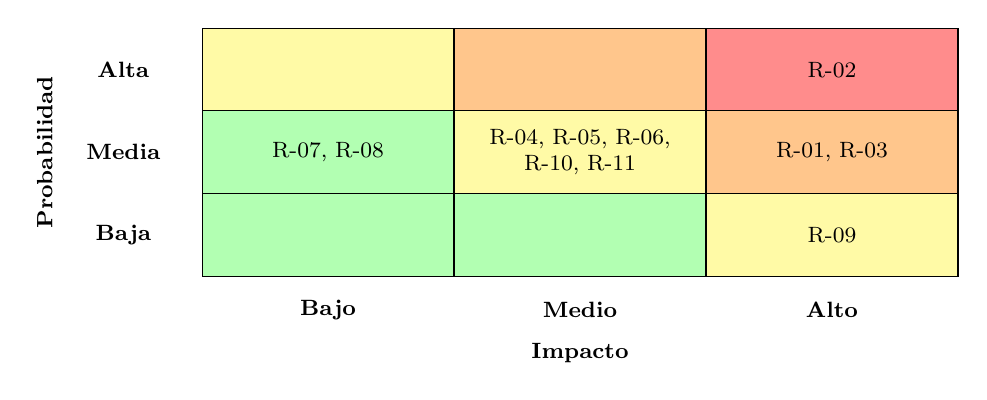
\begin{tikzpicture}[
      cell/.style={draw, minimum width=3.2cm, minimum height=1.05cm,
                   align=center, font=\footnotesize},
      lbl/.style={font=\footnotesize\bfseries}
    ]
    % Colores por nivel de exposición (probabilidad x impacto)
    \foreach \x/\y/\c/\t in {
        0/2/yellow!35/, 1/2/orange!45/, 2/2/red!45/{R-02},
        0/1/green!30/{R-07, R-08}, 1/1/yellow!35/{R-04, R-05, R-06,\\R-10, R-11}, 2/1/orange!45/{R-01, R-03},
        0/0/green!30/, 1/0/green!30/, 2/0/yellow!35/{R-09}} {
      \node[cell, fill=\c] at (3.2*\x, 1.05*\y) {\t};
    }
    \node[lbl] at (-2.6, 2.1) {Alta};
    \node[lbl] at (-2.6, 1.05) {Media};
    \node[lbl] at (-2.6, 0) {Baja};
    \node[lbl] at (0, -0.95) {Bajo};
    \node[lbl] at (3.2, -0.95) {Medio};
    \node[lbl] at (6.4, -0.95) {Alto};
    \node[lbl, rotate=90] at (-3.6, 1.05) {Probabilidad};
    \node[lbl] at (3.2, -1.5) {Impacto};
  \end{tikzpicture}
  \caption{Matriz de riesgos del proyecto.}
  \label{fig:plan-matriz-riesgos}
\end{figure}

Tres riesgos materializados merecen comentario por su enseñanza para la
planificación:

\begin{itemize}
  \item \textbf{B-04, exposición del entorno.} Los servicios locales de la
        base de datos publicaban sus puertos en todas las interfaces y el
        motor de contenedores insertaba reglas que se saltaban el cortafuegos,
        de modo que la base de datos de desarrollo, con credenciales conocidas
        y solo datos de prueba, fue accesible desde Internet durante
        aproximadamente una hora. Se corrigió con una regla persistente, se
        recrearon los volúmenes y se pasó a trabajar mediante un túnel SSH
        (ADR-010).
  \item \textbf{Fallos de control de acceso.} Las auditorías de la base de
        datos del CMS encontraron brechas reales, entre ellas una
        escalada de privilegios en el RBAC (B-05), comprobaciones que fallaban
        en abierto (B-06, B-23), una inyección SQL (B-24) y un escape de las
        denegaciones explícitas mediante delegación (B-47). El riesgo estaba
        previsto, y la mitigación ---auditoría obligatoria en todo cambio de
        base de datos--- es la que permitió detectarlos.
  \item \textbf{B-15, corte de conexión durante una tarea.} El trabajo quedó
        a medias y mezclado con una corrección de seguridad pendiente. La
        lección pasó al proceso: cada incremento se cierra con su propio
        \textit{commit}.
\end{itemize}

% ---------------------------------------------------------------------
\section{Gestión de la configuración}
\label{sec:plan-configuracion}

\begin{itemize}
  \item \textbf{Control de versiones.} Git, con un repositorio privado en
        GitHub (ADR-001). La
        rama principal es \texttt{main}; se trabaja en ramas por fase
        (\texttt{fase-1/base}, \texttt{fase-2/cms}, \texttt{fase-3/espanol}) que
        se fusionan en \texttt{main} al cerrar la fase, mediante
        \textit{pull request} cuando se requiere ejecutar la suite E2E en la
        CI. Los mensajes de \textit{commit} están en español y siguen
        \textit{Conventional Commits}~\cite{conventionalcommits} con el módulo
        como ámbito, por ejemplo \texttt{feat(cms): auditoría y búsqueda
        global (F2.6)}.
  \item \textbf{Base de datos como código.} El esquema se mantiene de forma
        declarativa en ficheros numerados, y las migraciones se generan a
        partir de ellos y se versionan en el repositorio. Nunca se modifica una
        migración ya aplicada: cada cambio es una migración nueva y no
        destructiva. Las pruebas pgTAP viven junto al esquema.
  \item \textbf{Configuración y secretos.} La configuración reutilizable está
        en ficheros \texttt{*.config.ts} validados con Zod y en variables de
        entorno públicas documentadas; los secretos solo se guardan en
        ficheros locales excluidos del repositorio o en las variables de la
        plataforma de despliegue.
  \item \textbf{Dependencias.} Un catálogo único de versiones para todo el
        monorepo, con el fichero de bloqueo versionado.
  \item \textbf{Entregas.} Cada fusión de una fase en \texttt{main} constituye
        una versión estable del producto (tabla~\ref{tab:plan-hitos}). La
        versión que se entrega con esta memoria se etiqueta en el repositorio
        (\texttt{v1.0-tfg}), de modo que el código entregado y el descrito
        coinciden.
\end{itemize}

% ---------------------------------------------------------------------
\section{Aseguramiento de calidad}
\label{sec:plan-calidad}

\subsection{Estándares y normas}

\begin{itemize}
  \item \textbf{Código}: TypeScript estricto, sin \texttt{any} sin
        justificar; \textit{lint} y formato automáticos; convenciones del
        repositorio para \textit{server functions}, formularios, clientes de
        base de datos y separación entre módulos de cliente y de servidor.
  \item \textbf{Comentarios}: guía propia de comentarios didácticos en
        español, con cabecera por fichero, documentación de las funciones
        exportadas y justificación obligatoria de toda decisión de seguridad.
  \item \textbf{Base de datos}: RLS obligatoria en toda tabla nueva,
        privilegios mínimos por verbo y por columna, y ninguna función con
        privilegios elevados sin controles explícitos.
  \item \textbf{Seguridad}: el estándar OWASP ASVS~\cite{owasp-asvs} sirve de
        referencia para los controles de autenticación, sesión y control de
        acceso.
  \item \textbf{Calidad del producto}: los requisitos no funcionales se
        alinean con las características del modelo ISO/IEC
        25010~\cite{iso25010}: seguridad (RNF-02, RNF-03), mantenibilidad y
        modularidad (RNF-04, RNF-05), flexibilidad e instalabilidad (RNF-07),
        capacidad de interacción (RNF-08) y eficiencia de desempeño (RNF-09).
  \item \textbf{Trazabilidad}: una matriz relaciona cada requisito con el
        código que lo implementa, las pruebas que lo verifican y la sección de
        la memoria que lo describe. Los puntos clave del código llevan
        etiquetas \texttt{[TFG]} que un script extrae a esa matriz.
\end{itemize}

\subsection{Verificación y validación}

Todo cambio pasa por la misma cadena de comprobaciones, declarada obligatoria
en las directrices del repositorio:

\begin{enumerate}
  \item comprobación de tipos, \textit{lint} y formato;
  \item controles automáticos del repositorio, tanto sobre el contenido
        como sobre las rutas de los ficheros;
  \item pruebas afectadas: unitarias, de base de datos (pgTAP) y E2E si se
        toca un flujo de usuario;
  \item revisión adversarial del cambio en dos pistas: calidad y
        arquitectura, y búsqueda de errores y fallos de seguridad;
  \item si el cambio afecta a la base de datos, auditoría adversarial de las
        políticas RLS en cuatro etapas: revisión estática, pruebas de ataque
        ejecutables entre clientes, refutación independiente de los hallazgos
        y corrección con pruebas de regresión;
  \item revisión de los comentarios del código; y
  \item actualización del progreso, la trazabilidad y, si procede, las
        decisiones y la bitácora.
\end{enumerate}

Las comprobaciones automatizables se repiten en la integración continua, en un
\textit{workflow} con tres trabajos: (1)~controles propios del TFG
(controles automáticos del repositorio, bloqueantes; informe de comentarios en inglés, informativo hasta
cerrar la F4); (2)~tipos, \textit{lint}, formato y pruebas unitarias; y
(3)~base de datos local, pruebas pgTAP y E2E con Playwright contra la
\textit{build} de test, que se ejecuta en las \textit{pull requests} hacia
\texttt{main} y bajo demanda.

\subsection{Criterios de aceptación y acciones correctoras}

Un incremento se acepta cuando cumple su criterio de «hecho», la cadena
anterior está en verde y el autor lo ha revisado. Se rechaza ---y se corrige
antes de continuar--- si una auditoría encuentra una brecha confirmada, si
alguna prueba deja de pasar o si los controles automáticos del repositorio
emiten un aviso. Cada incidencia se registra en la bitácora con su lección, y
cuando la lección es generalizable se convierte en una acción preventiva: una
regla nueva en las directrices, una variante más en un control automático
(B-01) o una prueba de regresión. A la fecha de corte la bitácora
recoge 60 incidencias, de las que 29 son de seguridad; todas las de gravedad alta están corregidas.


